\chapter{Oxidatie en reductie in de organische chemie}\label{ch:b1:organic-redox}

Een fles wijn die open blijft staan, wordt binnen enkele dagen azijn:
bacteriën gebruiken de zuurstof van de lucht om ethanol tot ethaanzuur te
oxideren. Een keton en de alcohol waaruit het ontstaat, verschillen twee
waterstofatomen --- en, goed geteld, twee elektronen. Organische
oxidaties en reducties lijken niet op de uitwisselingen van elektronen
tussen metaalionen van \cref{ch:b1:nernst}, omdat de elektronen reizen
met protonen of met hydride-ionen, maar de boekhouding is dezelfde. Dit
hoofdstuk kent \omterm{def:b1:organic-redox:oxidation-level}{oxidatieniveaus} toe aan koolstof, gebruikt ze om te
voorspellen wat elke alcohol bij oxidatie geeft, en introduceert de
hydridereagentia die carbonylverbindingen reduceren, met aandacht voor de
groepen die elk reagens ongemoeid laat.

\begin{recall}
\omterm{def:b1:nernst:oxidation-number}{Oxidatiegetallen}, \omterm{def:b1:nernst:couple}{halfreacties} en het kloppend maken van redoxvergelijkingen
staan in \cref{ch:b1:nernst}; de klassen van alcoholen en van
koolstofatomen in \cref{ch:b1:electronic-effects}; \omterm{def:b1:acetals-protection:hemiacetal}{acetalen} en de
\omterm{def:b1:acetals-protection:protecting-group}{bescherming} van carbonylgroepen in \cref{ch:b1:acetals-protection};
grignardaddities in \cref{ch:b1:organomagnesium}.
\end{recall}

\begin{omfigure}
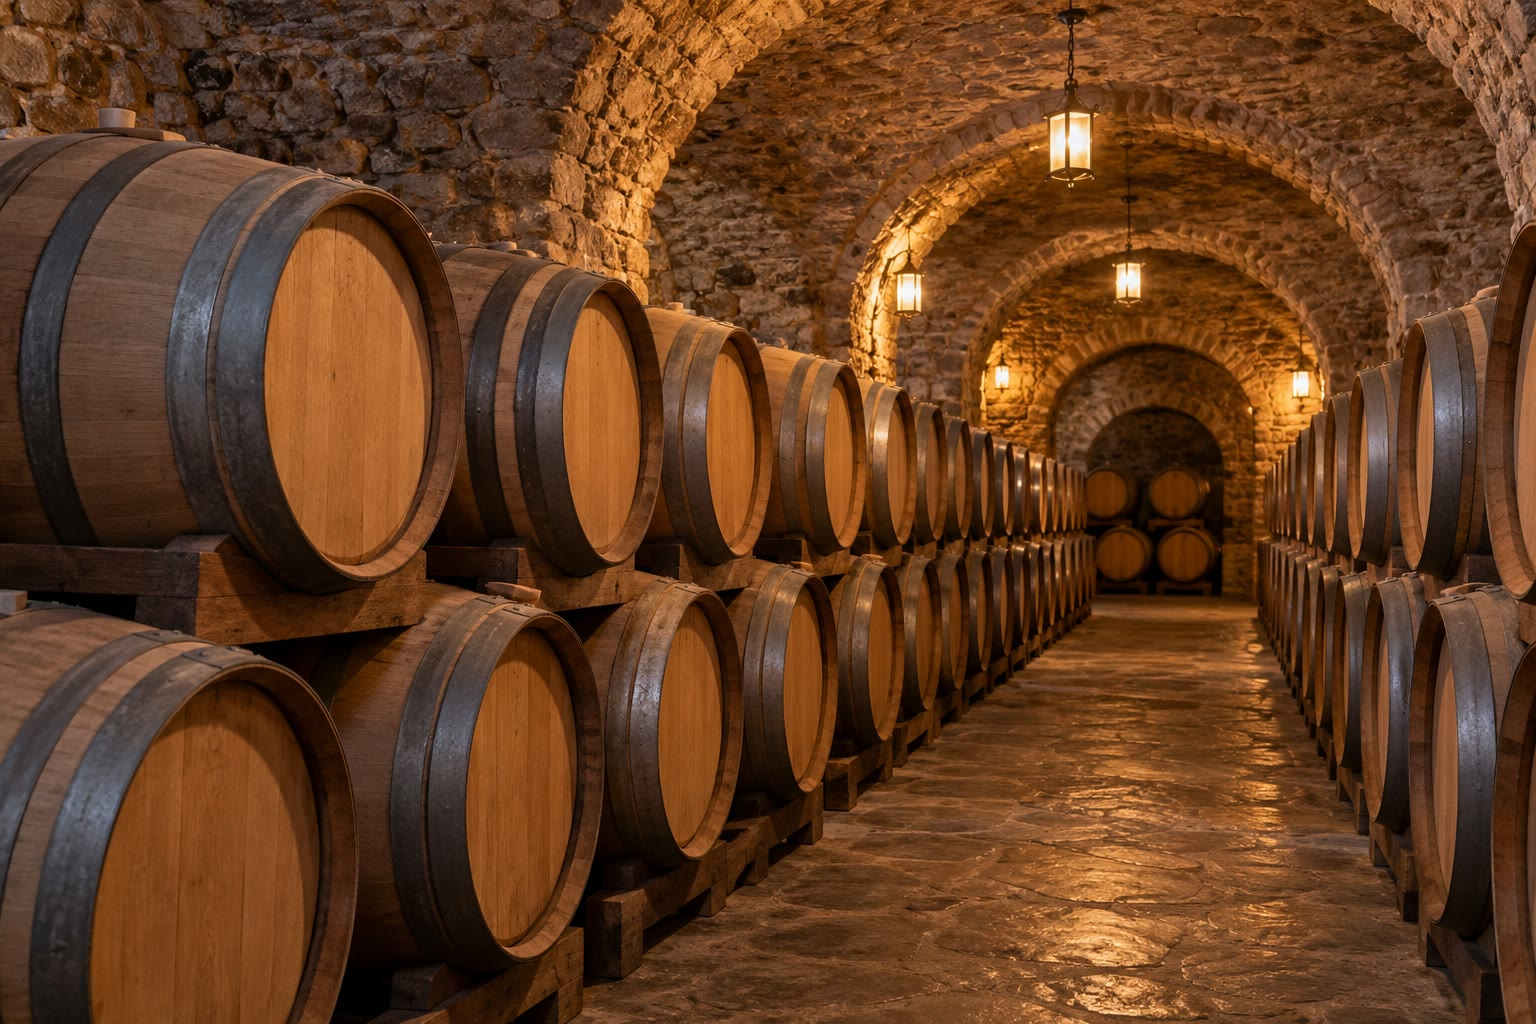
\includegraphics[width=0.58\linewidth]{images/book2/ai/b1-24-wine-cellar.jpg}

{\small Wijn die in een kelder rijpt. Buiten contact met de lucht behoudt
wijn zijn ethanol; blootgesteld aan lucht oxideren azijnzuurbacteriën hem
tot ethaanzuur.}
\end{omfigure}

\section{Oxidatieniveaus van koolstof}

\begin{definition}[Oxidatieniveau]\label{def:b1:organic-redox:oxidation-level}
Het \emph{oxidatieniveau}\index{oxidatieniveau} van een koolstofatoom is
zijn \omterm{def:b1:nernst:oxidation-number}{oxidatiegetal}, verkregen met de regels van
\cref{prop:b1:nernst:on-rules}: elke binding met een elektronegatiever
atoom (O, N, halogeen) telt $+1$, elke binding met waterstof $-1$, elke
binding met een ander koolstofatoom 0 (een dubbele binding telt twee
keer).
\end{definition}

\begin{proposition}[Oxidatiegetallen van koolstof]\label{prop:b1:organic-redox:on-of-carbon}
Het \omterm{def:b1:nernst:oxidation-number}{oxidatiegetal} van een koolstofatoom is gelijk aan (aantal bindingen
met O, N of halogenen) min (aantal bindingen met H). Binnen één familie
van verbindingen met hetzelfde koolstofskelet is alcohol $\to$ aldehyde of
keton $\to$ carbonzuur $\to$ koolstofdioxide een reeks oxidaties van elk
twee elektronen.
\end{proposition}

\begin{proof}
Verbreek elke binding en geef beide elektronen aan de elektronegatievere
partner: van H (minder elektronegatief dan C) wint koolstof een elektron,
lading $-1$ per C--H; aan O, N, halogenen (elektronegatiever) verliest
het er een, $+1$ per binding; C--C-bindingen worden gelijk verdeeld. Van
\ce{-CH2OH} ($-1$ voor een koolstofatoom gebonden aan één ander
koolstofatoom) naar \ce{-CHO} ($+1$) naar \ce{-COOH} ($+3$) stijgt het
getal bij elke stap met 2: twee elektronen.
\end{proof}

\begin{omfigure}
\begin{tikzpicture}[font=\small, >={Stealth}]
  \foreach \x/\f/\n in {0/\ce{CH4}/-4, 2.4/\ce{CH3OH}/-2, 4.8/\ce{HCHO}/0, 7.2/\ce{HCOOH}/+2, 9.6/\ce{CO2}/+4} {
    \node[draw, rounded corners, minimum width=1.5cm] at (\x,0) {\f};
    \node[below] at (\x,-0.5) {$\n$};
  }
  \foreach \x in {0.8,3.2,5.6,8.0} \draw[->, thick, omThm] (\x,0) -- ++(0.8,0);
  \node[omThm, above] at (4.8,0.5) {oxidatie: $-2\,\mathrm{e^-}$ (en $-2\,\ce{H+}$) per stap};
  \node[left] at (-0.9,-0.75) {OG van C:};
\end{tikzpicture}

{\small De \omterm{def:b1:organic-redox:oxidation-level}{oxidatieniveaus} van de familie met één koolstofatoom: methaan,
methanol, methanal, methaanzuur, koolstofdioxide. Elke pijl is een
oxidatie met twee elektronen; achterwaarts gelezen, een reductie.}
\end{omfigure}

\begin{method}[Een organische halfreactie kloppend maken]\label{met:b1:organic-redox:balance-organic-redox}
\begin{enumerate}
  \item Schrijf de organische \omterm{def:b1:nernst:couple}{oxidator} en \omterm{def:b1:nernst:couple}{reductor} met hetzelfde skelet
        op.
  \item Tel de elektronen uit de verandering van de \omterm{def:b1:nernst:oxidation-number}{oxidatiegetallen} van
        de koolstofatomen die veranderen (of eenvoudig: twee per verloren
        paar H, of per gewonnen O).
  \item Maak zuurstof kloppend met water, waterstof met \ce{H+}, lading
        met de elektronen.
\end{enumerate}
Ethanol naar ethaanzuur: \ce{CH3CH2OH + H2O -> CH3COOH + 4H+ + 4e-}.
Met aangezuurd dichromaat (\ce{Cr2O7^2- + 14H+ + 6e- -> 2Cr^3+ + 7H2O}),
drie ethanolmoleculen voor twee dichromaationen:
\ce{3CH3CH2OH + 2Cr2O7^2- + 16H+ -> 3CH3COOH + 4Cr^3+ + 11H2O}.
\end{method}

\section{Alcoholen oxideren}

\begin{proposition}[Wat alcoholen bij oxidatie geven]\label{prop:b1:organic-redox:alcohol-oxidation}
Een primaire alcohol \ce{RCH2OH} wordt geoxideerd tot het aldehyde
\ce{RCHO}, daarna (in water, met een sterke \omterm{def:b1:nernst:couple}{oxidator}) tot het carbonzuur
\ce{RCOOH}; een secundaire alcohol \ce{R2CHOH} tot het keton \ce{R2CO},
dat verdere oxidatie weerstaat; een tertiaire alcohol \ce{R3COH} wordt
niet geoxideerd zonder een C--C-binding te verbreken.
\end{proposition}

\begin{proof}
De oxidatie van de alcohol verwijdert het waterstofatoom van de OH en een
waterstofatoom van het carbinolkoolstofatoom, wat C=O vormt. Een tertiair
carbinolkoolstofatoom heeft zo'n waterstofatoom niet. Het aldehyde draagt
nog een H op het carbonylkoolstofatoom; in water is het gedeeltelijk
gehydrateerd, \ce{RCH(OH)2}, dat op dezelfde manier opnieuw geoxideerd
wordt tot \ce{RCOOH}. Een keton heeft geen H op dat koolstofatoom en
stopt.
\end{proof}

Sterke \omterm{def:b1:nernst:couple}{oxidatoren} in water --- aangezuurd kaliumdichromaat of
permanganaat --- oxideren primaire alcoholen tot zuren. Om bij het
aldehyde te stoppen, wordt het afgedestilleerd naarmate het ontstaat
(aldehyden koken lager dan de alcoholen waaruit ze ontstaan, omdat ze geen
O--H-waterstofbruggen hebben), of gebruikt men mildere, watervrije
reagentia, die in het deel van jaar~2 beschreven worden.

\begin{safety}{\ghs[5mm]{GHS03}\,\ghs[5mm]{GHS05}\,\ghs[5mm]{GHS06}\,\ghs[5mm]{GHS07}\,\ghs[5mm]{GHS08}\,\ghs[5mm]{GHS09}}
Kaliumdichromaat, de klassieke oranje \omterm{def:b1:nernst:couple}{oxidator} van alcoholen, behoort tot
de stoffen die kanker kunnen veroorzaken: het wordt alleen in kleine
hoeveelheden gehanteerd, met handschoenen en veiligheidsbril, en zijn
chroomafval wordt apart ingezameld; waar mogelijk verkiest men een minder
gevaarlijke \omterm{def:b1:nernst:couple}{oxidator}.
% ledger: ghs:K2Cr2O7
\end{safety}

\section{Carbonylverbindingen reduceren met hydriden}

\begin{definition}[Hydridedonor]\label{def:b1:organic-redox:hydride-donor}
Een \emph{hydridedonor}\index{hydridedonor} draagt een waterstofatoom met
zijn \omterm{def:b1:lewis-resonance-vsepr:lewis}{bindend paar}, \ce{H-}, over op een \omterm{def:b1:electronic-effects:nucleophile}{elektrofiel} koolstofatoom.
Natriumboorhydride \ce{NaBH4} en lithiumaluminiumhydride \ce{LiAlH4} zijn
\emph{complexe metaalhydriden}\index{complex metaalhydride}: het hydride
wordt vanuit het ion \ce{BH4-} of \ce{AlH4-} afgegeven, niet als vrij
ion.
\end{definition}

\begin{omfigure}
\setchemfig{atom sep=2.1em}
\schemestart
\chemfig{H_3B^{-}-[@{bh}]@{h}H}
\+
\chemfig{@{c}C(-[:150]R)(-[:210]R')=[@{co}]@{o}O}
\arrow{->}
\chemfig{C(-[:150]R)(-[:210]R')(-[2]H)-O^{-}}
\arrow{->[\ce{H2O}]}
\chemfig{C(-[:150]R)(-[:210]R')(-[2]H)-OH}
\schemestop
\chemmove{\draw[->, thick, shorten <=2pt, shorten >=3pt](bh) .. controls +(80:9mm) and +(180:7mm) .. (c);
          \draw[->, thick, shorten <=2pt, shorten >=2pt](co) .. controls +(90:6mm) and +(90:6mm) .. (o);}
\par\vspace{6pt}

{\small Reductie van een keton door boorhydride: een B--H-paar vormt de
nieuwe C--H-binding terwijl het $\pi$-paar van C=O naar de zuurstof gaat;
het \omterm{def:b1:alcohol-activation:alkoxide}{alkoxide} wordt geprotoneerd door het oplosmiddel (water of een
alcohol) of bij de opwerking. Elk \ce{BH4-} kan zijn vier waterstofatomen
een voor een afgeven.}
\end{omfigure}

\begin{proposition}[Bereik van de twee hydriden]\label{prop:b1:organic-redox:hydride-scope}
Natriumboorhydride, gebruikt in water of alcoholen, reduceert aldehyden
tot primaire alcoholen en ketonen tot secundaire alcoholen, en laat
esters, carbonzuren, amiden en dubbele C=C-bindingen ongemoeid.
Lithiumaluminiumhydride, gebruikt in droge ether, reduceert ook esters en
carbonzuren tot primaire alcoholen, en reageert heftig met water.
\end{proposition}

\begin{proof}
De Al--H-binding is sterker gepolariseerd dan de B--H-binding (aluminium
is minder elektronegatief dan boor), zodat \ce{AlH4-} een veel sterkere
\omterm{def:b1:organic-redox:hydride-donor}{hydridedonor} is, die de minder elektrofiele carbonylgroep van esters en
van carboxylaten kan aanvallen; dezelfde reactiviteit laat het reageren
met elk zuur waterstofatoom, ook dat van water. \ce{BH4-} reageert maar
langzaam met water en alcoholen, en valt alleen de meest elektrofiele
carbonylgroepen aan. Een geïsoleerde C=C-binding is niet \omterm{def:b1:electronic-effects:nucleophile}{elektrofiel} en
wordt door geen van beide gereduceerd.
\end{proof}

\section{Selectiviteit}

\begin{definition}[Chemoselectieve reactie]\label{def:b1:organic-redox:chemoselective}
Een \emph{chemoselectieve reactie}\index{chemoselectieve reactie} werkt in
op één functionele groep van een molecuul in aanwezigheid van andere die,
met een ander reagens, ook zouden kunnen reageren.
\end{definition}

\begin{omfigure}
\begin{tabular}{lcc}
\hline
groep & \ce{NaBH4} (alcohol als oplosmiddel) & \ce{LiAlH4} (droge ether) \\
\hline
aldehyde \ce{RCHO} & primaire alcohol & primaire alcohol \\
keton \ce{R2CO} & secundaire alcohol & secundaire alcohol \\
ester \ce{RCOOR} & geen reactie & twee alcoholen \\
carbonzuur \ce{RCOOH} & geen reactie (zout) & primaire alcohol \\
alkeen \ce{C=C} & geen reactie & geen reactie \\
\omterm{def:b1:acetals-protection:hemiacetal}{acetaal} & geen reactie & geen reactie \\
\hline
\end{tabular}

\smallskip
{\small Wat de twee hydriden reduceren. Natriumboorhydride is het
chemoselectieve reagens; lithiumaluminiumhydride, het krachtige.}
\end{omfigure}

\begin{example}[Een ketoester]\label{ex:b1:organic-redox:ketoester}
Ethyl-4-oxopentanoaat, \ce{CH3CO(CH2)2COOEt}, geeft met natriumboorhydride
ethyl-4-hydroxypentanoaat: alleen het keton wordt gereduceerd. Met
lithiumaluminiumhydride worden beide groepen gereduceerd:
pentaan-1,4-diol (en ethanol). Om alleen de ester te reduceren, moet het
keton eerst als \omterm{def:b1:acetals-protection:hemiacetal}{acetaal} beschermd worden (\cref{ch:b1:acetals-protection}).
\end{example}

\begin{inthelab}[Een keton reduceren]
Natriumboorhydride wordt in kleine porties toegevoegd aan een koude
oplossing van het keton in ethanol: de reactie is exotherm, en er borrelt
waterstof op door de trage reactie van het reagens met het oplosmiddel.
Na het roeren vernietigt verdund zuur de overmaat reagens (nog meer
waterstof: geen vlam in de buurt) en wordt de alcohol geëxtraheerd.
Lithiumaluminiumhydride daarentegen wordt alleen in droge ether onder een
inert gas gebruikt, en de overmaat ervan wordt met grote zorg
vernietigd.
\end{inthelab}

\section{Oefeningen}

\begin{exercise}[$\star$]\label{exo:b1:organic-redox:1}
Geef het \omterm{def:b1:nernst:oxidation-number}{oxidatiegetal} van elk koolstofatoom in ethanol, ethanal,
ethaanzuur, propanon en methaanzuur.
\end{exercise}

\begin{exercise}[$\star$]\label{exo:b1:organic-redox:2}
Wat geeft aangezuurd dichromaat met propaan-1-ol, propaan-2-ol en
2-methylpropaan-2-ol?
\end{exercise}

\begin{exercise}[$\star$]\label{exo:b1:organic-redox:3}
Schrijf de \omterm{def:b1:nernst:couple}{halfreacties} op van de koppels propanon/propaan-2-ol en
ethanal/ethanol in zuur milieu.
\end{exercise}

\begin{exercise}[$\star$]\label{exo:b1:organic-redox:4}
Wat geven natriumboorhydride en lithiumaluminiumhydride met butanal,
butanon, ethylbutanoaat en butaanzuur?
\end{exercise}

\begin{exercise}[$\star\star$]\label{exo:b1:organic-redox:5}
Maak de oxidatie van propaan-2-ol door permanganaat in zuur milieu
kloppend (\ce{MnO4-}/\ce{Mn^2+}) en bereken het volume permanganaat van
\qty{0.020}{mol/L} dat nodig is voor \qty{1.20}{g} alcohol ($M = \qty{60.0}{g/mol}$).
\end{exercise}

\begin{exercise}[$\star\star$]\label{exo:b1:organic-redox:6}
Hoe kan propanal uit propaan-1-ol verkregen worden zonder dat het verder
geoxideerd wordt? Gebruik de kookpunten: propaan-1-ol
\qty{97}{\celsius}, propanal \qty{48}{\celsius}.
% ledger: bp:propanal, bp:propan-1-ol
\end{exercise}

\begin{exercise}[$\star\star$]\label{exo:b1:organic-redox:7}
Schrijf het mechanisme op van de reductie van ethanal door \ce{BH4-} in
ethanol. Welk atoom van het product komt van het reagens?
\end{exercise}

\begin{exercise}[$\star\star$]\label{exo:b1:organic-redox:8}
De reductie van butanon met \ce{NaBH4} geeft een \omterm{def:b1:stereochemistry-in-depth:stereocentre}{chirale} alcohol. Is die
optisch actief? Waarom?
\end{exercise}

\begin{exercise}[$\star\star$]\label{exo:b1:organic-redox:9}
In de ademtest op alcohol die de politie vroeger gebruikte, werd oranje
dichromaat groen. Schrijf de reactie met ethanol op en verklaar de
kleurverandering.
\end{exercise}

\begin{exercise}[$\star\star\star$]\label{exo:b1:organic-redox:10}
Stel syntheses voor van: 2-methylbutaan-2-ol uit ethanal en een
\omterm{def:b1:organomagnesium:organometallic}{grignardreagens}, gevolgd door een oxidatie en een tweede grignardstap;
pentaan-3-ol uit propanal. Tel de oxidaties en reducties.
\end{exercise}

\begin{exercise}[$\star\star\star$]\label{exo:b1:organic-redox:11}
Reduceer alleen de estergroep van methyl-4-oxopentanoaat,
\ce{CH3CO(CH2)2COOCH3}. Plan de drie stappen met een \omterm{def:b1:acetals-protection:protecting-group}{bescherming} en geef
het product.
\end{exercise}

\begin{exercise}[$\star\star\star$]\label{exo:b1:organic-redox:12}
Toon met de \omterm{def:b1:nernst:oxidation-number}{oxidatiegetallen} en met de \omterm{def:b1:nernst:couple}{halfreactie} aan dat bij de
oxidatie van een primaire alcohol tot het zuur vier elektronen
uitgewisseld worden. Veralgemeen naar de oxidatie van methaan tot
koolstofdioxide.
\end{exercise}

\section{Probleem: van cyclohexanol naar adipinezuur}

\begin{problem}[{Weekendprobleem --- oxidatieniveaus in cyclohexanol,
cyclohexanon en adipinezuur, de oxidatie met salpeterzuur en haar
elektronen, een route met waterstofperoxide, en de massa distikstofoxide
die per ton adipinezuur vrijkomt}]
\label{pb:b1:organic-redox:1}
Adipinezuur, hexaandizuur \ce{HOOC(CH2)4COOH}, wordt op grote schaal
gemaakt voor de nylons, meestal door oxidatie van cyclohexanol (met
cyclohexanon) door salpeterzuur, waarbij distikstofoxide \ce{N2O}
vrijkomt, een krachtig broeikasgas. Molaire massa's (\unit{g/mol}):
\ce{C6H12O} 100.0, \ce{C6H10O} 98.0, \ce{C6H10O4} 146.0, \ce{N2O} 44.0,
\ce{HNO3} 63.0, \ce{H2O2} 34.0.

\medskip
\noindent\textbf{Deel I --- \omterm{def:b1:organic-redox:oxidation-level}{Oxidatieniveaus}.}
\begin{enumerate}
  \item Geef het \omterm{def:b1:nernst:oxidation-number}{oxidatiegetal} van elk koolstofatoom van cyclohexanol.
  \item Hetzelfde voor cyclohexanon.
  \item Hetzelfde voor adipinezuur.
  \item Welke koolstofatomen worden geoxideerd bij de overgang van
        cyclohexanol naar adipinezuur, en welke binding wordt verbroken?
  \item Hoeveel elektronen verliest één molecuul cyclohexanol?
  \item Waarom wordt cyclohexanon, een keton, hier toch verder
        geoxideerd?
\end{enumerate}

\medskip
\noindent\textbf{Deel II --- De route met salpeterzuur.}
\begin{enumerate}[resume]
  \item Schrijf de \omterm{def:b1:nernst:couple}{halfreactie} op van cyclohexanol naar adipinezuur in
        zuur milieu.
  \item Geef het \omterm{def:b1:nernst:oxidation-number}{oxidatiegetal} van N in \ce{HNO3} en in \ce{N2O}.
  \item Schrijf de \omterm{def:b1:nernst:couple}{halfreactie} \ce{HNO3}/\ce{N2O} op.
  \item Combineer ze; controleer dat je
        \ce{C6H12O + 2HNO3 -> C6H10O4 + N2O + 2H2O} krijgt.
  \item Hoeveel mol elektronen wordt er per mol adipinezuur uitgewisseld?
  \item Bereken de massa salpeterzuur die per ton adipinezuur verbruikt
        wordt.
\end{enumerate}

\medskip
\noindent\textbf{Deel III --- Een route met waterstofperoxide.}
\begin{enumerate}[resume]
  \item Schrijf de \omterm{def:b1:nernst:couple}{halfreactie} \ce{H2O2}/\ce{H2O} op.
  \item Schrijf de oxidatie van cyclohexanol door waterstofperoxide tot
        adipinezuur op en maak haar kloppend.
  \item Bereken de massa \ce{H2O2} per ton adipinezuur.
  \item Wat is het enige bijproduct? Waarom heet deze route groener?
  \item Waterstofperoxide moet door een \omterm{def:b1:elementary-steps:catalyst}{katalysator} geactiveerd worden.
        Verklaar met \cref{exo:b1:nernst:12} waarom een thermodynamisch
        begunstigde oxidatie er toch een nodig kan hebben.
  \item Wat zou natriumboorhydride met cyclohexanon doen? Schrijf de
        reactie op.
\end{enumerate}

\medskip
\noindent\textbf{Deel IV --- Massa's en het broeikasgas.}
\begin{enumerate}[resume]
  \item Bereken de hoeveelheid stof adipinezuur in één ton.
  \item Bereken de hoeveelheid \ce{N2O} die er via de route met
        salpeterzuur mee ontstaat.
  \item Bereken de massa cyclohexanol die per ton nodig is, bij een
        \omterm{def:b1:extent-q-and-k:fractional-extent}{rendement} van \qty{95}{\percent}.
  \item Geef de massa \ce{N2O} in ton die via de route met salpeterzuur
        per ton adipinezuur vrijkomt.
\end{enumerate}
\end{problem}
